%\documentclass[11pt]{article} % use larger type; default would be 10pt
%\usepackage[utf8]{inputenc} % set input encoding (not needed with XeLaTeX)
%
%%%% PAGE DIMENSIONS
%\usepackage{geometry} % to change the page dimensions
%\geometry{a4paper} % or letterpaper (US) or a5paper or....
%\newcommand{\tab}{\hspace*{2em}}
%
%%%% PACKAGES
%\usepackage{graphicx} % support the \includegraphics command and options
%\usepackage{wrapfig} % Figure wrapping
%% \usepackage[parfill]{parskip} % Activate to begin paragraphs with an empty line rather than an indent
%\usepackage{booktabs} % for much better looking tables
%\usepackage{array} % for better arrays (eg matrices) in maths
%\usepackage{paralist} % very flexible & customisable lists (eg. enumerate/itemize, etc.)
%\usepackage{verbatim} % adds environment for commenting out blocks of text & for better verbatim
%\usepackage{subfig} % make it possible to include more than one captioned figure/table in a single float
%\usepackage{url}
%\usepackage{enumerate}
%\usepackage{cleveref}  %cites figures intelligently
%\usepackage{import} % document structuring
%\usepackage{float}  %These two ensure that table position follows text by specifying {table}[H]
%\restylefloat{table}
%
%%CODE LISTINGS
%\usepackage{color}
%\usepackage{listings}
%
%\lstset{
%	tabsize=4,
%%	language=matlab,
%        	basicstyle=\scriptsize,
%%     	upquote=true,
%       	aboveskip={\baselineskip},
%        	columns=fixed,
%        	showstringspaces=false,
%        	extendedchars=true,
%        	breaklines=true,
%	prebreak = \raisebox{0ex}[0ex][0ex]{\ensuremath{\hookleftarrow}},
%	frame=single,
%        	showtabs=false,
%        	showspaces=false,
%        	showstringspaces=false,
%        	identifierstyle=\ttfamily,
%        	keywordstyle=\color[rgb]{0,0,1},
%        	commentstyle=\color[rgb]{0.133,0.545,0.133},
%        	stringstyle=\color[rgb]{0.627,0.126,0.941},
%	language=C++
%}
%
%%%% HEADERS & FOOTERS
%\usepackage{fancyhdr} % This should be set AFTER setting up the page geometry
%\pagestyle{fancy} % options: empty , plain , fancy
%\renewcommand{\headrulewidth}{0pt} % customise the layout...
%\lhead{}\chead{}\rhead{}
%\lfoot{}\cfoot{\thepage}\rfoot{}
%
%%%% SECTION TITLE APPEARANCE
%\usepackage{sectsty}
%\allsectionsfont{\sffamily\mdseries\upshape} % (See the fntguide.pdf for font help)
%\usepackage{titlesec}
%%\titleformat{\subsection}[runin]{\mdseries\bf}{\thesubsection}{1em}{}
%%\titleformat{\subsubsection}[runin]{\mdseries\bf\underline\large}{\thesubsection}{1 em}{\vspace{-5 pt}}
%
%\usepackage{footbib}
%
%% (This matches ConTeXt defaults)
%
%%%% ToC (table of contents) APPEARANCE
%%\usepackage[nottoc,notlof,notlot]{tocbibind} % Put the bibliography in the ToC
%\usepackage[titles,subfigure]{tocloft} % Alter the style of the Table of Contents
%\renewcommand{\cftsecfont}{\rmfamily\mdseries\upshape}
%\renewcommand{\cftsecpagefont}{\rmfamily\mdseries\upshape} % No bold!
%
%\begin{document}
%%% END Article customizations

\part{Background}
\section{Hardware}

\subsection{The Device}

\begin{wrapfigure}{R}{0.3\textwidth}
	\vspace{-40pt}
	\begin{center}
		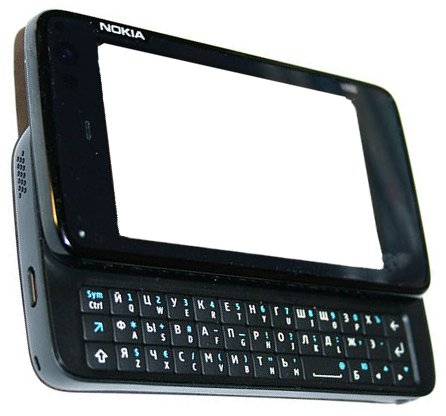
\includegraphics[width=0.3\textwidth]{../images/wiki_n900}
	\end{center}
	\vspace{-20pt}
	\caption{Front}
	\vspace{30pt}
	\begin{center}
		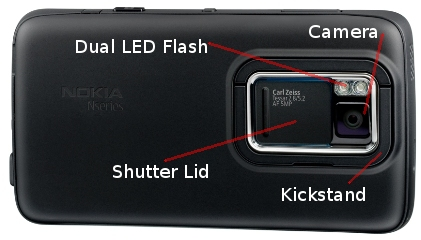
\includegraphics[width=0.3\textwidth]{../images/N900back}
	\end{center}
	\vspace{-20pt}
	\caption{Back}
\end{wrapfigure}

The N900 was Nokia's third attempt at producing an internet tablet phone after the initial success of the N810. Like it's predecessor it sported a hardware keyboard, a TFT touchscreen, accelerometer, 600 MHz ARM Corex CPU, and the same PowerVR SGX Graphics chip came with the iPhone 3GS.

At the time of it's release in 2009 it boasted competitive specs with every other smart phone on the market; supported flash (unlike the iPhone) and could multitask multiple apps at the same time. However it sold poorly due to unfamiliarity of its user interface and lack of 3rd party developers - indeed the only crowd it attracted was its already loyal Nokia fanbase from previous phones.

Despite these setbacks, the N900 has been heralded as one of the most well designed phones of its generation due to its open framework, native interation of Skype, fast boot time via Ubuntu's upstart daemon. It was also one of the first smartphone's to successfully port Android (the Nitdroid project) and could emulate other linux distros.

\subsection{Camera}
The Nokia N900 came with a 5 MegaPixel resolution, with dual LED flash, and a Carl Zeiss lens with a 5.2mm focal length, a fixed aperture (regulator of light) and focus minimum of 10cm.

The camera sensor uses CMOS technology rather than CCD, which makes it better suited for video than for photo due to CMOS having a larger framerate because of its rolling shutter. CMOS also holds the advantage of being good for night vision, which is a useful feature for a motion detecting application to have.

 It supports the following resolutions:
\begin{description}
\vspace{-5pt}
\item [Image:] (2576x1936),(2560x1440),(2048x1536),(1280x960)
\vspace{-5pt}
\item [Video:] (848x480),(640x480),(320x240) at 25fps
\end{description}

\section{Software}
\subsection{Maemo OS}
The Maemo operating system is a Debian-based platform developed by Nokia for its internet tablets. For the N900 the Maemo OS was in it's 5th revision (Maemo 5) codenamed 'Fremantle'. It is based mostly upon open-source code, though certain user-space elements such as telephone operations, taskbar applets, and system daemons were closed source much to the chagrin of the developers, but these were later 'opened' by keen developers after Nokia dropped it's over-the-air updates in 2011.

The desktop uses the Hildon GUI framework which is based on GTK. Software is installed via HAM Application Manager (UI) but also via the classic 'apt-get' command (from the terminal emultator Xterm) native to all Debian distributions supporting the aptitude package manager, since applications are compiled as .deb files as with all Debian flavours.

The media player uses the GStreamer multimedia framework to play videos....

For software development, applications can written in C, C++, Python, Ruby and Mono. Java applications can also be written but these require to a JME to be ran and gaining access to this from the phone is not facilitated easily.\\

{\small\bf For more detailed information regarding the Maemo OS and the Maemo community please consult page~\pageref{maemocomm} in the Further Background section of the Appendix.}

\subsection{Development Tools}
\subsubsection{Scratchbox and the Rootstrap device}
Scratchbox is a cross-compilation toolkit used for application development across Linux distributions aimed at mostly x86 and ARM architectures. For Maemo, this is the bare minimum required to develop applications since it comes shipped with the Maemo Application Development and Debugging Environment rootstrap device (or MADDE) required to build the .deb packages from source code.

The Rootstrap is effectively a directory containing all the same prebuilt ARM libraries and files that the phone has. Through a chrooted environment it is possible to install and run the same deb packages that Fremantle uses. \\A chrooted environment is when a new directory is set as 'the root' of a filesystem in order to run a process in a modified environment so that the process does not have access to files outside of its current root. To have access to system devices and utilities, chrooted environments often have  /dev (device), /sys (system), /proc (process) mounted and bound as well, giving the impression of a full-fledged system within a system.

\subsubsection{Qt Framework} 
Qt is an open-source cross-platform application framework developed by Nokia to facilitate in the creation of developing and testing apps.  It uses mainly C++ which even comes with the GCC toolchain, but also uses QML (Qt Meta Language) which is a Javascript-based language for building applications where fluid animations for widgets is desired. Qt also has bindings for Python, Ruby, Perl, Php, Java, and numerous other languages.\\

Though Qt was mostly Maemo and Symbian based, the next version of Qt (version 5, currently v4.7) will be aimed at Android, iOS, and Windows 8 mobile devices in the near future, making it possibly the tool for all applplication development in the future. This was due to Digia buying Qt from Nokia in 2012\cite{nokiasell}. This is a good thing, since it means that alot of applications will be extremely portable between platforms, and assuming that Project Tizen (see aforementioned Appendix page) has the same open framework as Maemo, may perhaps greatly extend the shelf life and portability of my own application.\\

\hspace{-20pt}{\bf Qt SDK}\\
The QtSDK holds many similarities with the Android SDK in that they both have GUI for creating layouts (Qt Designer), both access unique assets via a resource management system (QResources) , and both autogenerate events for widgets.\\

\hspace{-20pt}{\bf Android vs Qt}\\
In Android, to create a click event the SDK adds an OnClickEvent within the source file which acts as a listener for that particular widget. In Qt, to create a click event a Signal and Slot pair are created, where the widget gives the signal that it has been clicked, and the slot reacts to the signal by performing the code written by the userin the slot method. XXX
\\
Qt also has external modules for SQL, comes with it's own WebKit (similar to Android SDK), and allows for CSS stylesheets to be used when styling widgets. The webkit and SQL modules are external to the base modules because they must be specified in .pro file of the project by appending them to QT+=sql webkit.
\\
Differences from Android SDK are more due to the differences in their base languages (e.g. Java vs C++), where multiple inheritance is not allowed in Java, and chaining constructors are not allowed in C++.\\
User interfaces are split into three files: Ui source file, Ui header file, and Ui layout file. Like Android, the layout file is an XML-based heirarachy of tags which define layout order and parent/child widget. Unlike Android, the XML file itself cannot be editted from within the SDK (as of QtSDK version 2.1.2) and must be editted in the background by the Qt Designer interface.

Qt comes with it's own objects to help facilitate common tasks such as string handling via the QString class which lets the user manipulate strings without worrying about the memory management. Standard C++ libraries are included of course and if the user wishes to they can use the std::string module too (though they should remember to delete the string when it no longer needs to be used!)
\\Using Qt's Meta-Object Compiler (moc), a lot of files are autogenerated to handle Qt's C++ extensions. The moc tool simply reads the C++ header file and looks for Q\_Object macros so that it can handle signals and slots which are native to Qt.

Qt is well integrated with the Scratchbox toolkit and is set up to have automatic access to the libraries defined in the /usr/lib/ directory of the chrooted rootstrap device. To use a new library in Qt, one can either append the directory to the LIBS += variable in the .pro file, or can natively install the ARM package in the rootstrap device using xdpkg, a dpkg clone, in the rootstrap directory via the command:\\
/../QtSDK/Maemo/4.6.2/bin/mad-admin xdpkg -i <package\_name>\_armel.deb\\

\hspace{-20pt}{\bf Ubuntu vs Windows}\\
The QtSDK was developed in unix and ported over to windows. Linux binaries comes in 32-bit and 64-bit architectures, the latter of which is desirably faster than the former in terms of hardware emulation, building, packaging, and syntax detection.\\The Windows QtSDK is only 32 bit, mostly because of bugs in the Mingw64 project which aims to be a complete runtime environment for gcc which would support native Windows 64 and 32 bit binaries.\\
Naturally, the windows version of the QtSDK builds slower due to the smaller architecture limitation, however it is a great deal more stable as shown later in the report.\\

\hspace{-20pt}{\bf Hardware Device, Emulator}\\
The QtSDK supports testing the application on both a Hardware Device and the QEMU Emulator often pre-packaged with Scratchbox (though in recent versions Qt it has been the other way around). Due to the 32-bit restriction of the QtSDK on Windows machines, the emulator can be very slow when run, however this is the opposite when run in 64-bit on Linux.\\
For the duration of this project the code was tested on my own Hardware Device. This can be setup via regular networking over WLAN, or through USB networking. In order to do this the 'Madde Developer' app must be installed on the phone to enable this functionality, and to also ease in the generation and sharing of SSH keys between the phone and the SDK.

\subsubsection{Version Control}
The QtSDK also comes shipped with integrated version control with good support for most of the popular versioning control systems such as Git, Mercurial, Subversion, Perforce, CVS, and Bazaar.\\
Changes to a piece of code can be committed and pushed either through simple Keyboard combinations or access through a dropdown menu.\\
This was my first time using a versioning tool since I generally backup my last data on a USB stick, and my current data on Dropbox.
For this project I chose to use the newer Git distributed version control (DVCS) tool over the classic Subversion centralised version control (CVS) model, purely because this was a solo project and managing multiple commits to central server was not an issue, and also because Git is generally faster, since there is no need to communicate with a central server. I also used Dropbox to sync my current work as an extra precaution.\\
The repository I chose to host my work was BitBucket which is very similar to the classic GitHub and Launchpad, but due to its lack of online community and its shameless copying of GitHub's webpage layout, recieves very little traffic\cite{gitvs}. By this logic it would mean that access to the site would be swift and that even if I made my repository public sometime in the future, there would be very few occurences of interfering users hovering over my code and pointing out its flaws.
From the QtSDK, branches can be chosen through context menus and changes can be pushed to the server with an optional 'diff' screen to compare changes between versions.\\It should be noted that the SDK does not come shipped with Git and it is down to the user to install and setup Git repositories independently of the SDK, which can only access existing branches.\\Using the Git Handbook, I followed the 'master' 'develop' 'feature' 'hotfix' branching model where the 'master' branch holds the code for each stable release, 'develop' is branch for commiting new changes and features that are reasonably stable, but not yet ready for release. The 'feature' branch is branch that contains many branches for each new bleeding edge feature that is released  such as 'feature/avaraging\_method' or 'feature/subtract'. When these features have working prototypes they are then merged with the 'develop' branch. The 'hotfix' branch is a tiny branch that exists for quickly fixing small bugs that are found on a release.
\subsubsection{\LaTeX{}}
Previous reports of mine have often been written in OpenOffice or Abiword, but this time I decided to try LaTex.\\LaTex is an intuitive document creating language widely used in academia to produce proffesional papers and reports using the type-setting program Tex. It has native support for writing equations, producing tables, generating a table of contents, and simplifies bibliography management.\\Every part of the document is declared in a single marking tag which can declare a section, or subsection, or subsubsection, or paragraph, or subparagraph.
\\For trees I used the QTree package, and for bibliographies I didn't want the reader to have to constantly flip back and forth to a bibliography at the back, so I used the {\it footbib}\footnote{footbib - mirror.hmc.edu/ctan/macros/latex/contrib/footbib/footbib.pdf} package that placed references at the foot of the page whilst still maintaining the bibliography database. Footnotes were also frequently used whenever a citation was not likely to be quoted again.

\section{Literature Review}
Prior to development I was reading through a detailed review by Massimo Piccardi from the Computer Vision Research Group (CVRG) at the University of Technology, Sydney (UTS)\footnote{Background Sutraction Techniques - http://www-staff.it.uts.edu.au/~massimo/BackgroundSubtractionReview-Piccardi.pdf} on background subtractions. The review highlighted many common problems and pitfalls that would occur in trying to detect motion and how to overcome them.
Indeed on page~\pageref{autoexpose} I describe how I fell into the trap of not updating the exposure of the camera and thus not detecting changes in illumination.
Piccardi talks about how simple subtraction between one frame and the next is very sensitive to a threshold, since the background is simply the previous image. He goes on to mention a method of accumulating frames as a running averages to overcome this problem and you can see the implementation of both efforts on page~\pageref{proctechniques}.

Once I got to the stage where I needed to perform morphological operations I began to read about erosion and dilation techniques from H.E. Burdick's textbook Digital Imaging: Theory and Applications\footnote{Digital Imaging: Theory and Applications, H. E. Burdick, McGraw-Hill, 1997}. On chapter 5: Morphological Operations he discusses the uses of the different kernel masks neccesary for erosion, dilation, and what he deems "hit-and-miss operators". I expand more on the topic on page~\pageref{kernelmorph}.

For timelapse operations there was not many prior works that I could read from, mostly because the topic is quite self-explanatory. I did read a great deal about cron and the alarmd framework as mentioned in detail on page~\pageref{cronalarm}.

IP streaming was based on the gstreamer framework and I discuss that at length (with examples) on page~\pageref{gstreamertalk}.



%\end{document}